\section{HOPG-Probe}\label{sec:hopg-probe}
\subsection*{Struktur}
Hochorientierter pyrolyitscher Graphit (HOPG) ist kristalliner Kohlenstoff, wo Atome einer Schicht
auf einem hexagonalen Gitter geordnet sind, wodurch jedes Atom auf dieser zweidimensionalen 
Ebene von drei weiteren Atomen im Winkel von \SI{120}{\degree} verbunden ist. Zwei Schichten 
dieses Gitters sind versetzt übereinander geordnet (siehe \cref{fig:hopg-skizze}), weshalb durch die 
untere Ebene die Ladungsverteilung auf der Oberfläche beeinflusst wird.\par Wie in 
\cref{fig:hopg2} erkennbar ist bei den H-Atomen die Ladungsverteilung minimal und bei A-Atomen maximal.
Die Verteilung bei den B-Atomen befindet sich dazwischen, weshalb diese für das Mikroskop unsichtbar werden,
da ein RTM nicht unmittelbar die Oberflächentopographie messen kann, sondern die Aufenthaltswahrscheinlichkeit der 
Elektronen \cite[Kap.1 S.7]{rtm-leitpfaden}.

\begin{figure}[htb]
    \centering
    \begin{subfigure}{0.45\linewidth}
        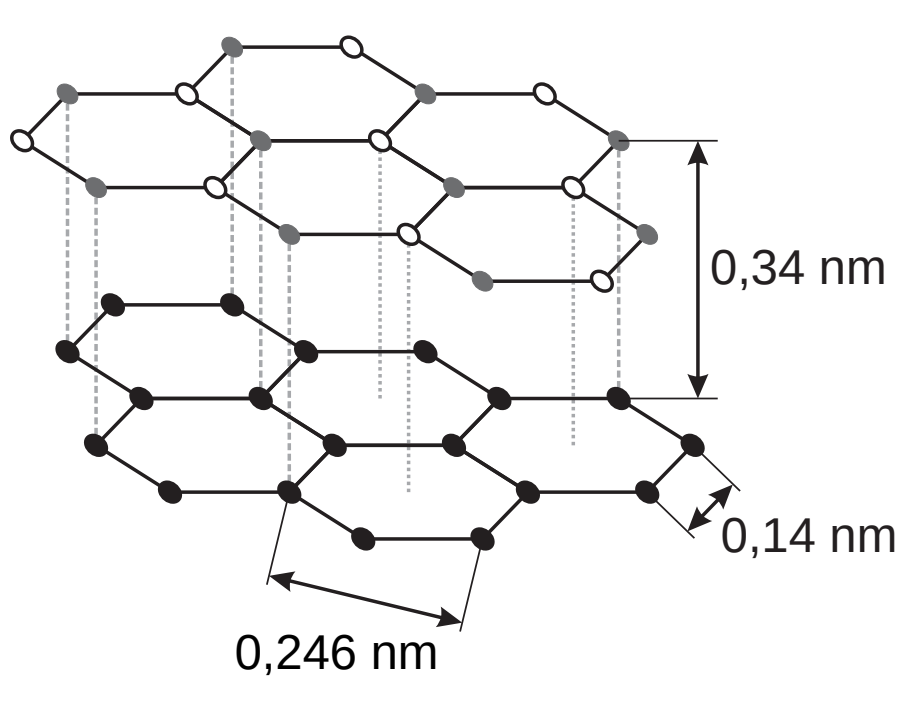
\includegraphics[width=\linewidth]{figs/hopg1.png}
        \caption{Seitenansicht.\cite[S.49]{skript}}
        \label{fig:hopg1}
    \end{subfigure}
    \hspace{0.5cm}
    \begin{subfigure}{0.45\linewidth}
        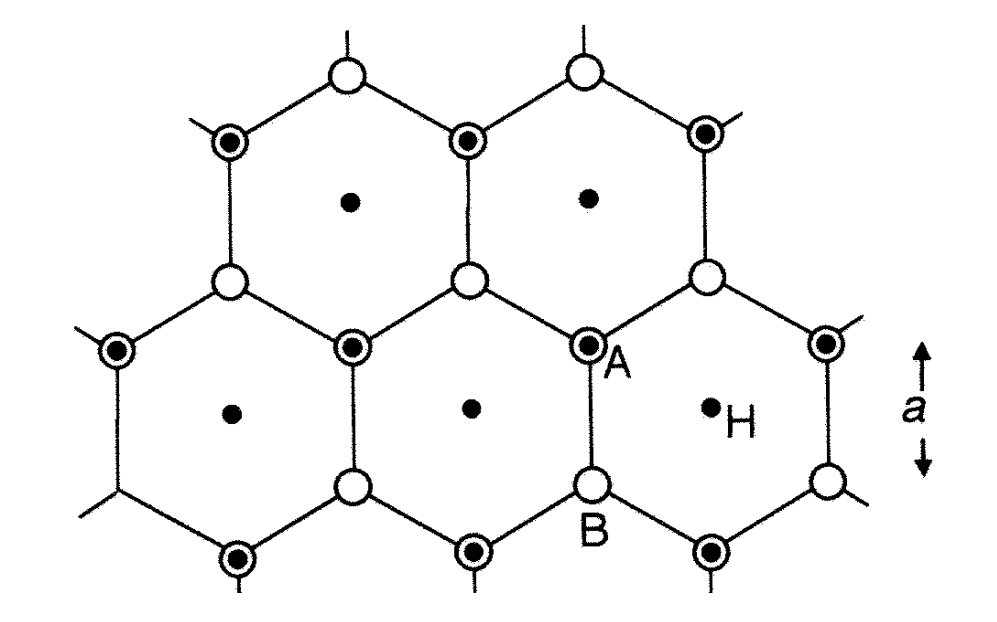
\includegraphics[width=\linewidth]{figs/hopg2.png}
        \caption{Obere Ansicht.\cite[Kap.1 S.17]{rtm-leitpfaden}}
        \label{fig:hopg2}
    \end{subfigure}
    \caption{Hochorientierter pyrolyitscher Graphit.}
    \label{fig:hopg-skizze}
\end{figure}

\subsection*{Vorbereitung}
Im Gegensatz zu Gold wird hier versucht, die atomare Struktur des Graphits aufzulösen. 
Dies erfordert hohe Präzision in der Durchführung und der Präparierung der Spitze. Der Platin-Iridium Draht
vor der Rasterung ist in \cref{fig:spitze_hopg_vorher_v2} abgebildet. Vorne ist eine dünne Spitze zur ekennen,
die sich für die Durchführung eignen sollte.

\begin{figure}[htb]
    \centering
    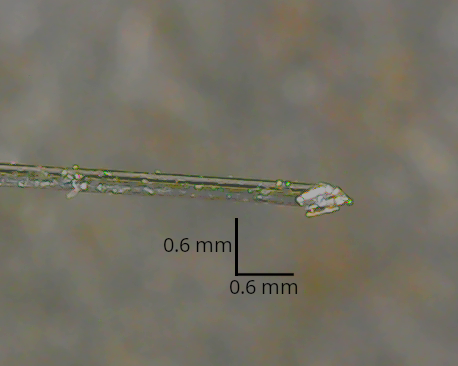
\includegraphics[width=0.5\linewidth]{figs/spitze_hopg_vorher_v2.png}
    \caption{Platin-Iridium Spitze vor Rasterung des HOPG.}
    \label{fig:spitze_hopg_vorher_v2}
\end{figure}

\begin{figure}[htb]
    \centering
    \begin{subfigure}{0.45\linewidth}
        \centering
        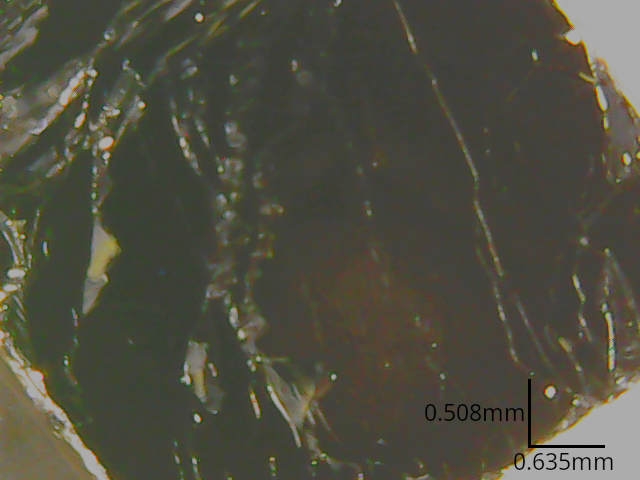
\includegraphics[width=\linewidth]{figs/hopg_skala1.png}
        \caption{Skala 1}
        \label{fig:hopg_skala1}
    \end{subfigure}
    \hspace{0.5cm}
    \begin{subfigure}{0.45\linewidth}
        \centering
        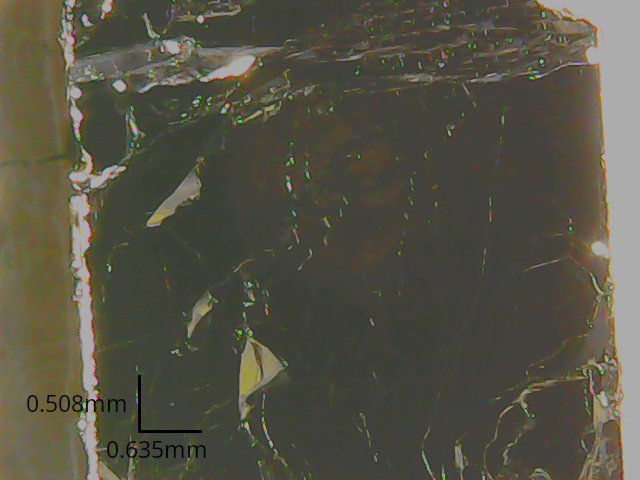
\includegraphics[width=\linewidth]{figs/hopg_skala2.png}
        \caption{Skala 2}
        \label{fig:hopg_skala2}
    \end{subfigure}
    \caption{USB-Mikroskop Aufnahmen von HOPG nach Abziehen der obersten Schicht.}
    \label{fig:usb_mikroskop_hopg}
\end{figure}

\begin{figure}[htb]
    \centering
    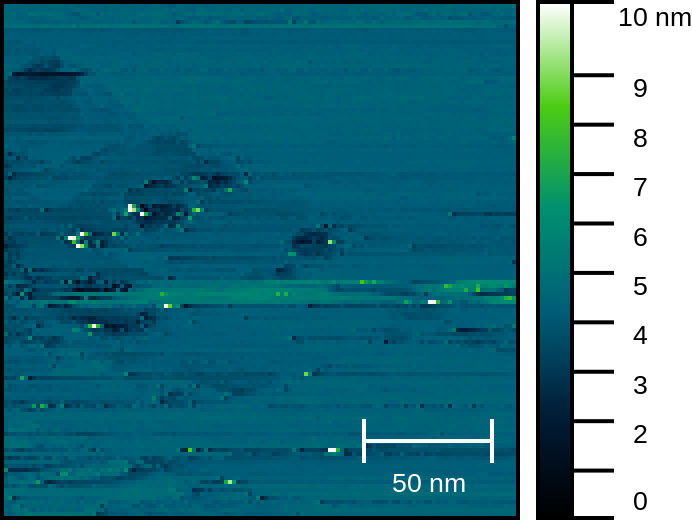
\includegraphics[width=0.6\linewidth]{figs/HOPG10558.png}
    \caption{HOPG und sonst?}
    \label{fig:hopg_rtm_weitaufnahme}
\end{figure}